\chapter{Θεωρία Ασαφών Συνόλων και Λογική}
\label{chap3}
Σε αυτό το κεφάλαιο παρουσιάζονται οι βασικές έννοιες της θεωρίας ασαφών συνόλων και της ασαφούς λογικής.
Οι \en{Klir} και \en{Yuan} \cite{KlirYuan} παρέχουν πιο αναλυτικές περιγραφές των αρχών της, ενώ οι \en{Nguyen} και \en{Walker} \cite{Nguyen} αναφέρονται σε πρακτικές εφαρμογές της. 
Η ασαφής λογική διευρύνει την κλασική θεωρία συνόλων και βοηθά στην ανάλυση δεδομένων που προέρχονται από βιοϊατρικές εφαρμογές στο πλαίσιο του Διαδικτύου των Πραγμάτων (\en{IoT}).

\section{Εισαγωγή}

Η μαθηματική λογική άρχισε να διαμορφώνεται στα μέσα του 19ου αιώνα, με σημαντικές συμβολές από τους \en{Boole} και \en{De Morgan}. Η προσπάθεια θεμελίωσης των Μαθηματικών ενσωμάτωσε τη φιλοσοφική λογική σε τυπικούς κανόνες. Μέσα σε αυτό το πλαίσιο, αναδείχθηκε η θεωρία συνόλων ως βασικό εργαλείο. Ορίζει σύνολα ως συλλογές αντικειμένων και στηρίζεται σε μια δυαδική σχέση μεταξύ ενός στοιχείου και ενός συνόλου: ανήκει ή δεν ανήκει.

Σύμφωνα με την κλασική θεωρία συνόλων, κάθε στοιχείο ενός συνόλου αναφοράς \(\Omega\) είτε βρίσκεται στο \(A\) είτε όχι. Η χαρακτηριστική συνάρτηση \(\chi_A\) διαχωρίζει ξεκάθαρα τα στοιχεία που ανήκουν στο \(A\) (τιμή 1) από αυτά που δεν ανήκουν (τιμή 0). Αυτό λειτουργεί καλά σε περιπτώσεις που οι έννοιες είναι σαφώς ορισμένες. Στη βιοϊατρική πράξη, όμως, συναντούμε ασάφεια. Συχνά, ένα στοιχείο ταιριάζει σε μια κατηγορία, αλλά όχι με απόλυτη βεβαιότητα.

Η θεωρία ασαφών συνόλων επεκτείνει τη δυαδική προσέγγιση και επιτρέπει ένα εύρος τιμών μεταξύ 0 και 1. Ο \en{Zadeh} \cite{Zadeh1965} παρατήρησε ότι πολλά σύνολα δεν έχουν καθαρά όρια και εισήγαγε την έννοια της συνάρτησης συμμετοχής. Με αυτόν τον τρόπο, αποτυπώνεται ο βαθμός στον οποίο κάθε στοιχείο συμμετέχει σε ένα ασαφές σύνολο, αντί για ένα απλό "ναι" ή "όχι".

Στα επόμενα τμήματα θα δούμε πώς αυτές οι συναρτήσεις συμμετοχής και οι πράξεις (συμπλήρωμα, τομή, ένωση) ορίζουν ένα πλαίσιο για την ασαφή λογική. Θα εστιάσουμε σε τρόπους με τους οποίους αυτή η προσέγγιση μπορεί να στηρίξει την επεξεργασία δεδομένων σε \en{IoT} εφαρμογές, κυρίως σε βιοϊατρικά περιβάλλοντα, όπου η αβεβαιότητα είναι συχνή.
Στα επόμενα κεφάλαια θα φανεί πώς αυτή η θεωρία μπορεί να εφαρμοστεί σε σύνθετες αναλύσεις δεδομένων, όπως τα μετρικά ομοιότητας ή απόστασης σε βιοϊατρικά σήματα από IoT συσκευές.

\section{Θεωρία Ασαφών Συνόλων}
Βασιζόμενοι στη συζήτηση για τους περιορισμούς των κλασικών (αυστηρών) συνόλων, προχωρούμε στον τυπικό ορισμό και την ερμηνεία των ασαφών συνόλων. Η βασική αρχή είναι ότι πολλές πραγματικές καταστάσεις περιλαμβάνουν ασάφεια και αβεβαιότητα, που δεν μπορούν να αποδοθούν ικανοποιητικά με ένα δυαδικό σχήμα "ανήκει/δεν ανήκει" \cite{Zadeh1965,KlirYuan}. Εντός αυτού του πλαισίου, ο \en{Zadeh} προέτεινε μια γενίκευση της κλασικής θεωρίας συνόλων, εισάγοντας την έννοια του βαθμού συμμετοχής κάθε στοιχείου.

\begin{figure}[h!] 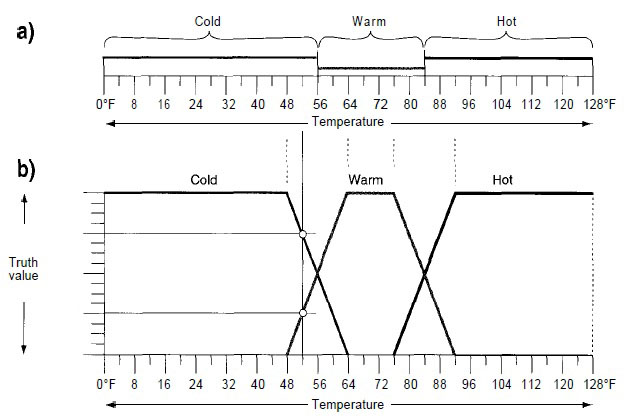
\includegraphics[scale=0.7]{images/fuzzy_logic1.jpg} \centering \caption{(\textlatin{a}) Παράδειγμα αυστηρού (\textlatin{crisp}) συνόλου, (\textlatin{b}) Παράδειγμα ασαφούς συνόλου.} \label{char_fun1} \end{figure}

\medskip

\begin{definition}
	\label{def:fuzzyset}
	\textbf{Ορισμός Ασαφούς Συνόλου.}\\
	Έστω \(\Omega\) ένα σύνολο αναφοράς. Ορίζουμε ένα \emph{ασαφές σύνολο} \(A \subseteq \Omega\) ως το διατεταγμένο ζεύγος
	\begin{equation}
	\label{eq:1}
	A = \{(x,\ \mu_{A}(x)) \mid x \in \Omega,\ \mu_{A}: \Omega \rightarrow [0,1]\},
	\end{equation}
	όπου \(\mu_{A}(x)\) είναι η \emph{συνάρτηση συμμετοχής} του \(x\) στο \(A\). Η τιμή \(\mu_{A}(x)\) μπορεί να λάβει οποιαδήποτε πραγματική τιμή στο διάστημα \([0,1]\), εκφράζοντας σε ποιον βαθμό το στοιχείο \(x\) ανήκει στο ασαφές σύνολο \(A\).
\end{definition}

Στο Σχήμα~\ref{char_fun1}\,(\textlatin{b}) παρουσιάζεται η γραφική απεικόνιση μιας τέτοιας συνάρτησης συμμετοχής, σε αντιδιαστολή με το αυστηρό (\(\{0,1\}\)) σχήμα του κλασικού συνόλου στο Σχήμα~\ref{char_fun1}\,(\textlatin{a}). 

\medskip
Σε περιπτώσεις όπου το ασαφές σύνολο \(A\) είναι \emph{διακριτό}, μπορούμε να το συμβολίσουμε ως:
\begin{equation}
\label{eq:2}
A = \sum_{i=1}^{n} \mu_{A}(x_{i})/x_{i},
\end{equation}
όπου το σύμβολο \(\sum\) υποδηλώνει την "ένωση" όλων των στοιχείων και \(\mu_{A}(x_{i})/x_{i}\) σημαίνει ότι το στοιχείο \(x_{i}\) ανήκει στο \(A\) με βαθμό συμμετοχής \(\mu_{A}(x_{i})\). Σημειώνεται ότι ο χαρακτήρας "/" δεν δηλώνει διαίρεση αλλά συμβατική σημείωση που απαντάται συχνά στη βιβλιογραφία \cite{DuboisPrade1980}.

\medskip
Αντίστοιχα, όταν το \(A\) είναι \emph{συνεχές}, γράφεται:
\begin{equation}
\label{eq:3}
\int_{x} \mu_{A}(x)/x,
\end{equation}
όπου το ολοκλήρωμα \(\int\) καταδεικνύει την "ένωση" σε έναν συνεχόμενο χώρο αναφοράς \(\Omega\).

\begin{definition}
	\label{def:normal}
	\textbf{Κανονικό Ασαφές Σύνολο.}\\
	Ένα ασαφές σύνολο \(A\) καλείται \emph{κανονικό} (\textlatin{normal}) εάν η συνάρτηση συμμετοχής του φτάνει το 1 για τουλάχιστον ένα στοιχείο:
	\begin{equation}
	\label{eq:4}
	\max_{x \in \Omega} \mu_{A}(x) = 1.
	\end{equation}
	Με άλλα λόγια, υπάρχει τουλάχιστον ένα \(x \in \Omega\) που ανήκει στο \(A\) με πλήρη βαθμό συμμετοχής.
\end{definition}

\begin{definition}
	\textbf{Πληθικότητα Ασαφούς Συνόλου (\en{Cardinality}).}\\
	Για ένα πεπερασμένο σύνολο αναφοράς \(\Omega\), ορίζουμε την \emph{πληθικότητα} του ασαφούς συνόλου \(A\) ως:
	\begin{equation}
	\label{eq:5}
	|A| = \sum_{x \in \Omega} \mu_{A}(x).
	\end{equation}
	Αντίστοιχα, η \emph{σχετική πληθικότητα} του \(A\) ως προς \(\Omega\) είναι:
	\begin{equation}
	\|A\| = \frac{|A|}{|\Omega|}.
	\end{equation}
	Οι έννοιες αυτές ποσοτικοποιούν το πόσο "μεγάλο" είναι το ασαφές σύνολο, λαμβάνοντας υπόψη τους μη-δυαδικούς βαθμούς συμμετοχής \cite{KlirYuan}.
\end{definition}

Στον Πίνακα~\ref{tab:part} συνοψίζονται μερικές από τις πιο διαδεδομένες μορφές συναρτήσεων συμμετοχής. Οι παραμετρικές εκφράσεις (π.χ. \(a, b, c, d, \sigma\)) καθορίζουν το σχήμα της συνάρτησης, καθιστώντας τη χρήσιμη για διαφορετικές εφαρμογές. Για παράδειγμα, η τριγωνική και η τραπεζοειδής μορφή προσφέρουν απλές, κομμάτι-γραμμικές προσεγγίσεις, ενώ η \textlatin{Gaussian} υποστηρίζει ομαλότερες μεταβάσεις \cite{Ross2010}.

\begin{table}[h!]
    \centering
    \begin{tabularx}{\textwidth}{>{\hsize=.4\hsize}X X >{\hsize=.5\hsize}X}
        \textbf{Συνάρτηση} & \textbf{Τύπος} & \textbf{Γραφική απεικόνιση} \\
        \hline
         \textbf{Τριγωνική} 
         & \(\displaystyle \mu_{A}(x) = \max\Bigl[\min\Bigl\{\tfrac{x-a}{b-a}, \tfrac{c-x}{c-b}\Bigr\}, 0\Bigr]\)
         & \begin{center}
             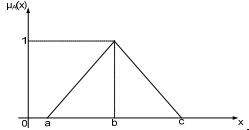
\includegraphics[scale=0.7]{images/trig.jpg}
           \end{center} \\
         \textbf{Τραπεζοειδής}
         & \(\displaystyle \mu_{A}(x) = \max\Bigl[\min\Bigl\{\tfrac{x-a}{b-a}, 1, \tfrac{d-x}{d-c}\Bigr\}, 0\Bigr]\)
         & \begin{center}
             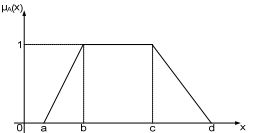
\includegraphics[scale=0.7]{images/trapez.jpg}
           \end{center}\\
         \textbf{\textlatin{Gaussian}}
         & \(\displaystyle \mu_{A}(x) = e^{-\bigl(\tfrac{x-b}{\sigma}\bigr)^2}\)
         & \begin{center}
             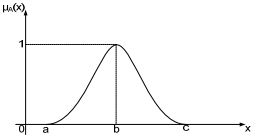
\includegraphics[scale=0.7]{images/gauss.jpg}
           \end{center}\\
         \textbf{Καμπανοειδής}
         & \(\displaystyle \mu_{A}(x) = \Bigl(1 + \Bigl|\tfrac{x-c}{a}\Bigr|^{2b}\Bigr)^{-1}\)
         & \begin{center}
             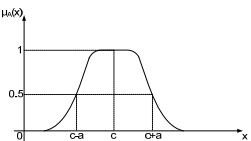
\includegraphics[scale=0.7]{images/bell.jpg}
           \end{center}\\
         \textbf{Σιγμοειδής}
         & \(\displaystyle \mu_{A}(x) = \bigl(1 + e^{-\,a\,(x-c)}\bigr)^{-1}\)
         & \begin{center}
             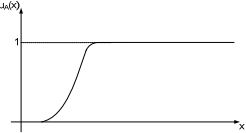
\includegraphics[scale=0.7]{images/sigm.jpg}
           \end{center}\\
    \end{tabularx}
    \caption{Παραδείγματα κοινών συναρτήσεων συμμετοχής (βάσει \cite{KlirYuan1995,Ross2010}).}
    \label{tab:part}
\end{table}

\medskip
Οι διαφορετικές μορφές παρουσιάζουν πλεονεκτήματα ανάλογα με την εκάστοτε εφαρμογή· για παράδειγμα, η τριγωνική συναρτήση συχνά χρησιμοποιείται για συστήματα με απλούς υπολογισμούς, ενώ η \textlatin{Gaussian} είναι κατάλληλη όταν οι μεταβάσεις πρέπει να είναι πιο ομαλές \cite{Zadeh1965,Ross2010}.

\medskip
Σε επόμενη ενότητα, θα ασχοληθούμε με τις πράξεις επί των ασαφών συνόλων (τομή, ένωση, συμπλήρωμα) και θα αναδείξουμε πώς αυτές γενικεύουν τις αντίστοιχες κλασικές πράξεις, καλύπτοντας μεγαλύτερη γκάμα εφαρμογών που χαρακτηρίζονται από αβεβαιότητα ή \emph{μερική αλήθεια}. Έτσι, το θεωρητικό υπόβαθρο που περιγράφεται σε αυτό το κεφάλαιο αποτελεί τη βάση για την περαιτέρω ανάπτυξη ασαφών συστημάτων και μεθόδων συμπερασμού.

\section{Τελεστές Ασαφούς Συνολοθεωρίας}

Στην κλασική θεωρία συνόλων, οι πράξεις της τομής, της ένωσης και του συμπληρώματος καθορίζουν πώς τα σύνολα αλληλεπιδρούν. Στο πλαίσιο των ασαφών συνόλων, οι ίδιες πράξεις γενικεύονται, ώστε να διαχειρίζονται βαθμούς συμμετοχής \cite{Zadeh1965,KlirYuan}. Η επιλογή της κατάλληλης ασαφούς πράξης εξαρτάται από τις απαιτήσεις της εφαρμογής.  

\subsection{Βασικές Σχέσεις: Κενό, Υποσύνολο, Ισότητα}

Όπως στην κλασική θεωρία, ορίζουμε το κενό ασαφές σύνολο \(\emptyset\) όταν η συνάρτηση συμμετοχής είναι μηδενική παντού:
\begin{equation}
    A = \emptyset \;\;\; \Longleftrightarrow \;\;\; \mu_{A}(x) = 0, \;\; \forall x\in \Omega.
\end{equation}
Δύο ασαφή σύνολα \(A\) και \(B\) θεωρούνται ίσα αν έχουν την ίδια συνάρτηση συμμετοχής:
\begin{equation}
    A = B \;\;\; \Longleftrightarrow \;\;\; \mu_{A}(x) = \mu_{B}(x), \;\; \forall x \in \Omega.
\end{equation}
Ο ορισμός του υποσυνόλου διαφοροποιείται από την κλασική περίπτωση ως εξής:
\begin{equation}
    A \subseteq B \;\;\; \Longleftrightarrow \;\;\; \mu_{A}(x) \leq \mu_{B}(x), \;\; \forall x \in \Omega,
\end{equation}
υποδηλώνοντας ότι ένα ασαφές σύνολο \(A\) είναι υποσύνολο ενός ασαφούς συνόλου \(B\) εάν η συνάρτηση συμμετοχής του είναι μικρότερη ή ίση αυτής του \(B\), για κάθε αντικείμενο του συνόλου αναφοράς \(\Omega\). Αυτό συχνά επιτρέπει στο \(A\) και το \(B\) να έχουν το ίδιο πλήθος στοιχείων, αλλά με διαφορετικούς βαθμούς συμμετοχής \cite{DuboisPrade1980}.

\subsection{Ασαφές Συμπλήρωμα}

Το συμπλήρωμα ενός ασαφούς συνόλου \(A\) ορίζεται από μια συνάρτηση 
\(
C : [0,1] \rightarrow [0,1],
\)
η οποία, για κάθε \(x \in \Omega\), αντιστοιχίζει τον βαθμό συμμετοχής \(\mu_A(x)\) στο βαθμό συμμετοχής του \(x\) στο συμπληρωματικό σύνολο \(\bar{A}\) \cite{Ross2010}. 
Οι συναρτήσεις αυτές οφείλουν να ικανοποιούν τα εξής αξιώματα:
\begin{enumerate}[label=(\textbf{\en{C}\arabic*)}, align=left, leftmargin=1em]
    \item Οριακές συνθήκες --- \(C(0) = 1\) και \(C(1) = 0\), δηλαδή ο ασαφής τελεστής \(C\) συμπεριφέρεται όπως το τυπικό συμπλήρωμα στις οριακές συνθήκες.
    \item Μονοτονία --- \(a<b \implies C(a) \geq C(b),\ \ \forall a,b \in [0,1]\), δηλαδή ο τελεστής \(C\) πρέπει να είναι μια φθίνουσα συνάρτηση.
\end{enumerate}
\par
Πέρα από τα παραπάνω, συνήθως λαμβάνονται υπόψη και άλλα 2 αξιώματα, τα οποία περιορίζουν την κλάση των συναρτήσεων που ικανοποιούν τα παραπάνω.
\begin{enumerate}[label=(\textbf{\en{C}\arabic*)}, align=left, leftmargin=1em]
    \setcounter{enumi}{2}
    \item Συνέχεια --- Ο τελεστής \(C\) να είναι συνεχής.
    \item Ενέλιξη --- \(C(C(a)) =a\)
\end{enumerate}

Οι πιο διαδεδομένες συναρτήσεις συμπληρώματος φαίνονται στον Πίνακα~\ref{tab:supp}, με κεντρικότερη:
\begin{equation}
    C(x) = 1 - x.
\end{equation}

\begin{table}[h!]
    \centering
    \begin{tabularx}{\textwidth}{X X}
        \textbf{Συνάρτηση} & \textbf{Τύπος}\\
        \hline
        \rule{0pt}{5ex}\textbf{Πρότυπο}
        & \(\displaystyle C(x) = 1 - x\) \\
        \rule{0pt}{5ex}\textbf{Κατώφλι}
        & \(\displaystyle C(x) = \begin{cases}
              1, & x \leq \tau \\
              0, & \text{αλλιώς}
           \end{cases}, \quad \tau \in [0,1]\)\\
        \rule{0pt}{5ex}\textbf{Συνημιτονοειδές}
        & \(\displaystyle C(x) = \frac{1 + \cos(\pi x)}{2}\)\\
        \textbf{\textlatin{Sugeno}}
        & \(\displaystyle C(x) = \frac{1 - x}{1 + \lambda x}, \quad \lambda > -1\)\\
        \textbf{\textlatin{Yagar}}
        & \(\displaystyle C(x) = (1 - x^w)^{\tfrac{1}{w}}, \quad w>0\)
    \end{tabularx}
    \caption{Συναρτήσεις ασαφούς συμπληρώματος \cite{Zadeh1965,DuboisPrade1980}.}
    \label{tab:supp}
\end{table}

\subsection{Ασαφής Τομή (\en{t-norm})}

Η ασαφής τομή δύο ασαφών συνόλων \(A\) και \(B\) δίνεται από έναν \textit{δυαδικό τελεστή} 
\[
T : [0,1]\times[0,1] \to [0,1],
\]
γνωστό και ως \textit{\en{triangular norm}} (\textit{\en{t-norm}}). 
Έχει καθιερωθεί πως οι συναρτήσεις, οι οποίες σχετίζονται με την πράξη της τομής, χρειάζεται να ικανοποιούν τα εξής αξιώματα, για \(a,b,c,d \in [0,1]\):
\begin{enumerate}[label=(\textbf{\en{T}\arabic*)}, align=left, leftmargin=1em]
    \item Οριακές συνθήκες --- \(T(1,a) = a\)
    \item Μονοτονία --- \(a \leq c\ \wedge\ b \leq d  \implies T(a,b) \leq T(c,d)\)
    \item Αντιμεταθετική ιδιότητα --- \( T(a,b) = T(b,a) \)
    \item Προσεταιριστική ιδιότητα --- \( T(a,T(b,c)) =T(T(a,b),c) \)
\end{enumerate}
Η απλούστερη και πιο διαδεδομένη συνάρτηση τομής είναι:
\begin{equation}
    T(a,b) = \min(a,b),
\end{equation}
όμως υπάρχουν εναλλακτικές, όπως το \(\textit{αλγεβρικό γινόμενο}\) ή η \(\textit{φραγμένη διαφορά}\) (Πίνακας~\ref{tab:inter}).
Στις πρακτικές εφαρμογές του IoT, η επιλογή της συνάρτησης \en{t-norm} είναι καθοριστική για τη συνδυαστική αξιολόγηση πολλών μετρικών από διαφορετικούς αισθητήρες (π.χ. συνδυάζοντας “ήπια” κατώφλια πίεσης και θερμοκρασίας).

\begin{table}[h!]
    \centering
    \begin{tabularx}{\textwidth}{X X}
        \textbf{Συνάρτηση} & \textbf{Τύπος}\\
        \hline
        \rule{0pt}{5ex}\textbf{Πρότυπο}
        & \(\displaystyle T(a,b) = \min(a,b)\)\\
        \rule{0pt}{5ex}\textbf{Δραστικό γινόμενο}
        & \(\displaystyle T(a,b) = \begin{cases}
              a, & b=1\\
              b, & a=1\\
              0, & \text{αλλιώς}
        \end{cases}\)\\
        \textbf{Αλγεβρικό γινόμενο}
        & \(\displaystyle T(a,b) = a\cdot b\)\\
        \textbf{Φραγμένη διαφορά}
        & \(\displaystyle T(a,b) = \max(0,a + b - 1)\)
    \end{tabularx}
    \caption{Παραδείγματα \en{t-norm} (ασαφούς τομής)}
    \label{tab:inter}
\end{table}

\subsection{Ασαφής Ένωση (\en{t-conorm})}

Ανάλογα, η ασαφής ένωση ορίζεται από έναν \textit{\en{t-conorm}} (\textit{\en{triangular conorm}}), 
\[
S : [0,1]\times[0,1] \to [0,1],
\]
που πληρεί αντίστοιχα αξιώματα (οριακές συνθήκες, μονοτονία, αντιμεταθετικότητα, προσεταιριστικότητα) \cite{DuboisPrade1980}. Ο τυπικός ορισμός είναι:
\begin{equation}
    S(a,b) = \max(a,b),
\end{equation}
αλλά και εδώ υπάρχουν διάφορες εναλλακτικές (Πίνακας~\ref{tab:un}). 
Συστήματα ελέγχου ή συστήματα υποστήριξης απόφασης συχνά χρησιμοποιούν ελαστικότερες \en{t-conorm} για να συνδυάσουν πολλαπλά κριτήρια με διαφορετικούς βαθμούς ικανοποίησης \cite{Zadeh1965,KlirYuan}. Για παράδειγμα, το αλγεβρικό άθροισμα επιτρέπει πιο ομαλή συνάθροιση των επιμέρους βαθμών συμμετοχής.

\begin{table}[h!]
    \centering
    \begin{tabularx}{\textwidth}{X X}
        \textbf{Συνάρτηση} & \textbf{Τύπος}\\
        \hline
        \rule{0pt}{5ex}\textbf{Πρότυπο}
        & \(\displaystyle S(a,b) = \max(a,b)\)\\
        \rule{0pt}{5ex}\textbf{Δραστικό άθροισμα}
        & \(\displaystyle S(a,b) = \begin{cases}
              a, & b=0\\
              b, & a=0\\
              1, & \text{αλλιώς}
        \end{cases}\)\\
        \textbf{Αλγεβρικό άθροισμα}
        & \(\displaystyle S(a,b) = a + b - ab\)\\
        \textbf{Φραγμένο άθροισμα}
        & \(\displaystyle S(a,b) = \min(1, a + b)\)
    \end{tabularx}
    \caption{Βασικοί τελεστές ασαφούς ένωσης (\en{t-conorm})}
    \label{tab:un}
\end{table}

\subsection{Ασαφής Συνεπαγωγή}

Η ασαφής συνεπαγωγή δίνεται από έναν \textit{δυαδικό τελεστή}
\[
J : [0,1]\times[0,1] \to [0,1],
\]
γνωστό και ως \textit{ασαφή συνεπαγωγή} (\textit{\en{fuzzy implication}}).
Έχει καθιερωθεί πως οι συναρτήσεις, οι οποίες σχετίζονται με την πράξη της συνεπαγωγής, χρειάζεται να ικανοποιούν τα εξής αξιώματα, για \(a,b,c,d \in [0,1]\):
\begin{enumerate}[label=(\textbf{\en{I}\arabic*)}, align=left, leftmargin=1em]
    \item Οριακές συνθήκες --- \(J(0,a) = 1\) και \(J(1,a) = a\)
    \item Μονοτονία στο δεύτερο όρισμα --- \(b \leq d \implies J(a,b) \leq J(a,d)\)
    \item Αντιμονοτονία στο πρώτο όρισμα --- \(a \leq c \implies J(c,b) \leq J(a,b)\)
\end{enumerate}

Η απλούστερη και πιο διαδεδομένη συνάρτηση συνεπαγωγής είναι:
\begin{equation}
    J(a,b) = \max(1-a,b),
\end{equation}
όμως υπάρχουν εναλλακτικές, όπως η \textit{συνεπαγωγή \en{Lukasiewicz}} ή η \textit{συνεπαγωγή \en{Mamdani}} (Πίνακας~\ref{tab:imply}) \cite{Zadeh1965,KlirYuan,Ross2010}.

\begin{table}[h!]
    \centering
    \begin{tabularx}{\textwidth}{X X}
       \textbf{Συνάρτηση} & \textbf{Τύπος}\\
       \hline
       \rule{0pt}{3ex} \textbf{\textlatin{Zadeh}}
       & \(a \rightarrow b = \max\,(1-a,\;\min\,(a,b))\) \\
       \rule{0pt}{3ex} \textbf{\textlatin{Lukasiewicz}}
       & \(a \rightarrow b = \min\,(1,\,1-a+b)\) \\
       \rule{0pt}{3ex} \textbf{\textlatin{Mamdani}}
       & \(a \rightarrow b = \min\,(a,b)\) \\
       \rule{0pt}{3ex} \textbf{\textlatin{Larsen}}
       & \(a \rightarrow b = a\,b \) \\
       \rule{0pt}{3ex} \textbf{\textlatin{Standard Strict}}
       & \(\displaystyle a \rightarrow b = \begin{cases}
           1, & a \leq b \\
           0, & \text{αλλιώς}
       \end{cases}\) \\
       \rule{0pt}{3ex} \textbf{\textlatin{G\"odel}}
       & \(\displaystyle a \rightarrow b = \begin{cases}
           1, & a \leq b \\
           b, & \text{αλλιώς}
       \end{cases}\) \\
       \rule{0pt}{3ex} \textbf{\textlatin{Goguen}}
       & \(\displaystyle a \rightarrow b = \begin{cases}
           1, & a \leq b \\
           \tfrac{b}{a}, & \text{αλλιώς}
       \end{cases}\) \\
       \rule{0pt}{3ex} \textbf{\textlatin{Yager}}
       & \(\displaystyle a \rightarrow b = \begin{cases}
           1, & a=b=0\\
           b^{\,a}, & \text{αλλιώς}
       \end{cases}\) \\
       \rule{0pt}{3ex} \textbf{\textlatin{Kleene-Dienes}}
       & \(a \rightarrow b = \max(1-a,\,b)\) \\
       \rule{0pt}{3ex} \textbf{\textlatin{Reichenbach}}
       & \(a \rightarrow b = 1 - a + ab\)
    \end{tabularx}
    \caption{Ενδεικτικοί τελεστές ασαφούς συνεπαγωγής \cite{KlirYuan1995,Ross2010}}
    \label{tab:imply}
\end{table}

\noindent
Συμπερασματικά, οι ασαφείς πράξεις και οι τελεστές συνεπαγωγής παρέχουν τη θεωρητική βάση για την επεξεργασία βαθμών συμμετοχής σε σύνθετα προβλήματα συλλογιστικής, ελέγχου και λήψης αποφάσεων. Στα επόμενα κεφάλαια, θα εξετάσουμε πώς οι διάφορες επιλογές (π.χ. τύπος συμπληρώματος, μορφή \en{t-norm}, είδος συνεπαγωγής) επηρεάζουν συγκεκριμένες εφαρμογές, από ασαφή ερωτήματα αναζήτησης σε περιβάλλοντα \en{IoT} έως ασαφή συστήματα ελέγχου σε βιοϊατρικές εφαρμογές.
\subsection{Συνδυασμοί Ασαφών Πράξεων}

Στην θεωρία συνόλων, οι πράξεις της τομής και της ένωσης είναι δυικές ως προς την πράξη του συμπληρώματος. Αυτή η σχέση εκφράζεται με τους νόμους \en{De Morgan}, οι οποίοι δηλώνουν ότι το συμπλήρωμα της τομής δύο συνόλων είναι ίσο με την ένωση των συμπληρωμάτων τους, και αντίστροφα:
\begin{align}
\begin{split}
    \overline{A \cap B} = \overline{A} \cup \overline{B} \\
    \overline{A \cup B} = \overline{A} \cap \overline{B} \\
\end{split}
\end{align}

Προφανώς, μόνο ορισμένοι συνδυασμοί των αντίστοιχων πράξεων στην ασαφή συνολοθεωρία ικανοποιούν την δυικότητα αυτή.
\begin{definition}
Μια \en{t-norm} και μια \en{t-conorm} είναι δυικές ως προς το ασαφές συμπλήρωμα \(C\) αν και μόνο εάν:
\begin{align}
\begin{split}
C(T(a,b)) = S(C(a),C(b)) \\
C(S(a,b)) = T(C(a),C(b))
\end{split}
\end{align}
\end{definition}

Στον Πίνακα \ref{tab:comb}, δίνονται τριάδες ασαφών πράξεων, στις οποίες η τομή και η ένωση είναι δυικές ως προς το συμπλήρωμα. Οι συνδυασμοί αυτοί χρησιμοποιούνται για να διατηρούν την ιδιότητα της δυικότητας σε ασαφή συστήματα.

\begin{table}[h!]
    \centering
    \begin{tabularx}{\textwidth}{X X X}
        \textbf{Τομή} & \textbf{Ένωση} & \textbf{Συμπλήρωμα} \\
        \hline
         \rule{0pt}{3ex}\(\min(a,b)\) & \(\max(a,b)\) & \(1-x\) \\
         \rule{0pt}{3ex}\(ab\) & \(a + b - ab\) & \(1-x\) \\
         \rule{0pt}{3ex}\(\max(0, a+b-1)\) & \(\min(1, a + b)\) & \(1-x\) \\
         \rule{0pt}{5ex}\(\left\{
            \begin{array}{ll}
                  a & b = 1 \\
                  b & a = 1 \\
                  0 & \textit{αλλιώς}\\
            \end{array} 
            \right.\) & \(\left\{
            \begin{array}{ll}
                  a & b = 0 \\
                  b & a = 0 \\
                  1 & \textit{αλλιώς}\\
            \end{array} 
            \right.\) & \(1-x\)
    \end{tabularx}
    \caption{Συνδυασμοί ασαφών πράξεων που διατηρούν τη δυικότητα}
    \label{tab:comb}
\end{table}

  Η θεωρία ασαφών συνόλων και λογική, όπως παρουσιάστηκε σε αυτό το κεφάλαιο, παρέχουν το απαραίτητο θεωρητικό υπόβαθρο για εφαρμογές που απαιτούν σταδιακούς βαθμούς συμμετοχής και αντιμετώπιση αβεβαιότητας.
  Οι ορισμοί των ασαφών συνόλων, οι συναρτήσεις συμμετοχής και οι τελεστές (συμπλήρωμα, τομή, ένωση, συνεπαγωγή) επιτρέπουν την αποτελεσματική μοντελοποίηση περίπλοκων συνθηκών,
  τη συνένωση πληροφοριών από πολλαπλούς αισθητήρες και την εκτέλεση κανόνων μερικής αλήθειας. 
  Στο επόμενο κεφάλαιο θα δούμε πώς αυτές οι αρχές μπορούν να επεκταθούν στη διαμόρφωση εξειδικευμένων \emph{\textlatin{fuzzy metrics}} με προσαρμοσμένες συναρτήσεις συμμετοχής,
  διευκολύνοντας ασαφή αναζήτηση σε δεδομένα \textlatin{IoT}, ιδίως σε βιοϊατρικές εφαρμογές όπου η αβεβαιότητα είναι συχνή.